\documentclass[../../../../../../Assignments.tex]{subfiles}

% \documentclass{book}
% \usepackage{pgfplots}
% \pgfplotsset{compat=1.17}


\begin{document}
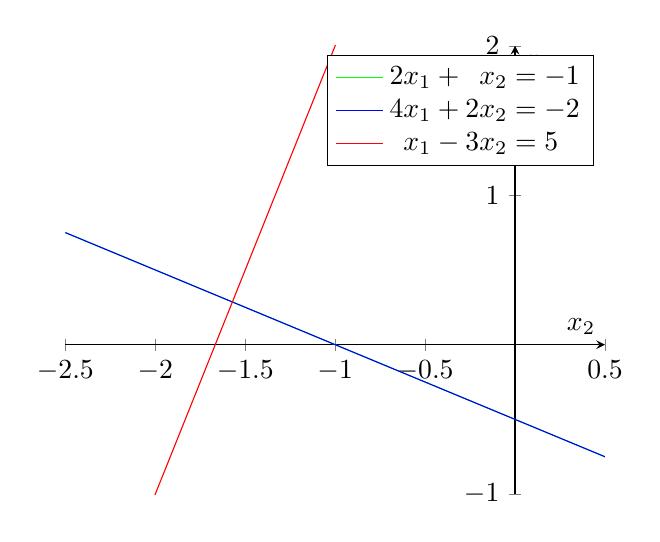
\begin{tikzpicture}
    \begin{axis}[
        axis lines = center,
        samples=10,
        xlabel = \(x_2\),
        xmin=-2.5, xmax=0.5,
        ylabel = \(x_1\),
        ymin=-1, ymax=2,
        legend cell align={left},
    ]
        \addplot[green]{-0.5 - 0.5 * x};
        \addlegendentry{\(2x_1 + \phantom{3}x_2 = -1\)};

        \addplot[blue]{-0.5 - 0.5 * x};
        \addlegendentry{\(4x_1 + 2x_2 = -2\)};

        \addplot[red]{3 * x + 5};
        \addlegendentry{\(\phantom{4}x_1 - 3x_2 = 5\)};
    \end{axis}
\end{tikzpicture}
\end{document}
